% !TeX root = ../../paper.tex

Questionnaire responses were scored following the anchors of the administered form: all items use 7-point scales, and items~1 (``How aware were you of the real world\ldots''), 11 (``I still paid attention to the real environment'') and 13 (``I felt like I was just perceiving pictures'') were reverse-coded so that higher values always indicate more presence. Item~6 needed no recoding, as its response anchors already run from ``did not feel present'' to ``felt present''. Subscale scores are item means: general presence (item~8), spatial presence (items 3, 6, 9, 10, 13), involvement (items 1, 7, 11, 14), and experienced realism (items 2, 4, 5, 12), following the IPQ structure~\cite{Schubert.2001}.

Descriptive statistics cover all twelve playthroughs (haptic $n=7$, baseline $n=5$); the paired analysis uses the five participants who completed both conditions. Table~\ref{tab:ipq-results} summarizes both.

\begin{table}[t]
  \caption{IPQ subscale scores (1--7), reported as $M$ ($SD$) over all playthroughs; $\Delta$, $t$, and $d_z$ from the five complete pairs.}
  \label{tab:ipq-results}
  \small
  \setlength{\tabcolsep}{4.5pt}
  \begin{tabular}{lccccc}
    \toprule
    Subscale & Haptic & Baseline & $\Delta$ & $t(4)$, $p$ & $d_z$ \\
    \midrule
    General presence     & 5.71 (0.49) & 2.40 (0.55) & $+3.20$ & 6.53, .003 & 2.92 \\
    Spatial presence     & 6.09 (0.70) & 2.96 (0.50) & $+3.12$ & 6.87, .002 & 3.07 \\
    Involvement          & 5.04 (0.88) & 2.15 (0.63) & $+2.65$ & 7.39, .002 & 3.30 \\
    Experienced realism  & 4.36 (1.17) & 2.25 (0.47) & $+2.05$ & 5.05, .007 & 2.26 \\
    \bottomrule
  \end{tabular}
\end{table}

\begin{figure}[t]
  \centering
  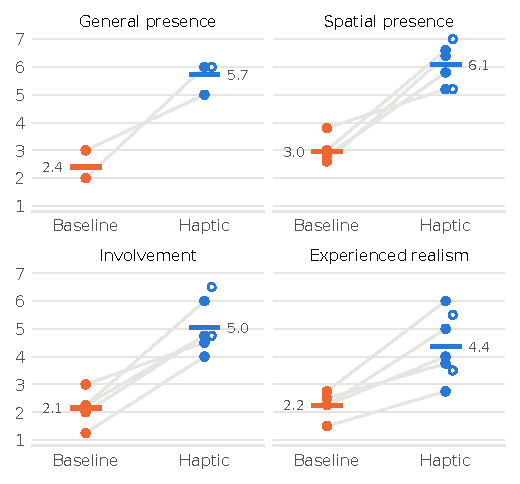
\includegraphics[width=\columnwidth]{figures/ipq_subscales}
  \caption{IPQ subscale scores per condition. Gray lines connect the two playthroughs of the same participant ($n=5$); open circles are the two participants who played only the haptic condition; horizontal ticks mark condition means over all playthroughs.}
  \Description{Four slope panels, one per IPQ subscale. In each panel every connecting line rises steeply from the baseline condition to the haptic condition.}
  \label{fig:ipq-subscales}
\end{figure}

The pattern is unambiguous in direction: every one of the five paired participants scored the haptic playthrough higher than the baseline on every subscale (Figure~\ref{fig:ipq-subscales}). The exact Wilcoxon signed-rank test accordingly yields $W=0$ with $p=.0625$ for all four subscales---the smallest $p$-value attainable with five pairs, so the test cannot reach the conventional .05 threshold regardless of effect size. Paired $t$-tests, reported in Table~\ref{tab:ipq-results} for orientation, are significant throughout, with effect sizes ($d_z$ between 2.3 and 3.3) that are very large by any convention; given the sample size we treat these numbers as descriptive rather than confirmatory. The direction of the effect did not depend on presentation order: the per-participant differences were positive for both baseline-first and haptic-first participants (spatial presence differences ranged from $+1.4$ to $+3.8$).

\begin{figure}[t]
  \centering
  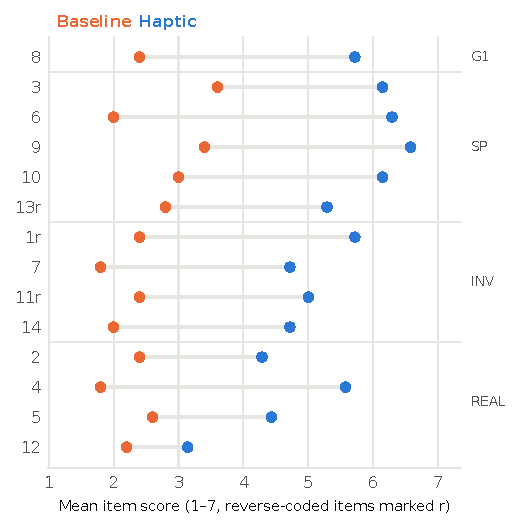
\includegraphics[width=\columnwidth]{figures/ipq_items}
  \caption{Mean score per IPQ item and condition (haptic $n=7$, baseline $n=5$), grouped by subscale; reverse-coded items are marked~r.}
  \Description{Dumbbell chart of the fourteen IPQ items. The haptic mean lies to the right of the baseline mean on every item; the gap is smallest for item 12.}
  \label{fig:ipq-items}
\end{figure}

At the item level (Figure~\ref{fig:ipq-items}), the largest gaps appear on item~6 (``I did not feel present in the virtual space'', $+4.3$ after recoding), item~4 (consistency with real-world experience, $+3.8$), and item~1 (awareness of the real surroundings, $+3.3$)---the items closest to what a haptic proxy manipulates. The smallest gap is on item~12 (``The virtual world seemed more realistic than the real world'', $+0.9$), which stayed low in both conditions; unsurprisingly, touching gummy worms does not make a virtual cabin outrank reality. Baseline scores were strikingly low overall (subscale means between 2.2 and 3.0), which we return to in the discussion.

\todoin{Optional: one short paragraph of behavioral observations---refusals, startle reactions, memorable comments during play.}
